\documentclass[]{article}
\usepackage{lmodern}
\usepackage{amssymb,amsmath}
\usepackage{ifxetex,ifluatex}
\usepackage{fixltx2e} % provides \textsubscript
\ifnum 0\ifxetex 1\fi\ifluatex 1\fi=0 % if pdftex
  \usepackage[T1]{fontenc}
  \usepackage[utf8]{inputenc}
\else % if luatex or xelatex
  \ifxetex
    \usepackage{mathspec}
    \usepackage{xltxtra,xunicode}
  \else
    \usepackage{fontspec}
  \fi
  \defaultfontfeatures{Mapping=tex-text,Scale=MatchLowercase}
  \newcommand{\euro}{€}
\fi
% use upquote if available, for straight quotes in verbatim environments
\IfFileExists{upquote.sty}{\usepackage{upquote}}{}
% use microtype if available
\IfFileExists{microtype.sty}{%
\usepackage{microtype}
\UseMicrotypeSet[protrusion]{basicmath} % disable protrusion for tt fonts
}{}
\usepackage{graphicx}
\makeatletter
\def\maxwidth{\ifdim\Gin@nat@width>\linewidth\linewidth\else\Gin@nat@width\fi}
\def\maxheight{\ifdim\Gin@nat@height>\textheight\textheight\else\Gin@nat@height\fi}
\makeatother
% Scale images if necessary, so that they will not overflow the page
% margins by default, and it is still possible to overwrite the defaults
% using explicit options in \includegraphics[width, height, ...]{}
\setkeys{Gin}{width=\maxwidth,height=\maxheight,keepaspectratio}
\ifxetex
  \usepackage[setpagesize=false, % page size defined by xetex
              unicode=false, % unicode breaks when used with xetex
              xetex]{hyperref}
\else
  \usepackage[unicode=true]{hyperref}
\fi
\hypersetup{breaklinks=true,
            bookmarks=true,
            pdfauthor={Tyler Neylon},
            pdftitle={Self-Replicating Functions},
            colorlinks=true,
            citecolor=blue,
            urlcolor=blue,
            linkcolor=black,
            pdfborder={0 0 0}}
\urlstyle{same}  % don't use monospace font for urls
\setlength{\parindent}{0pt}
\setlength{\parskip}{6pt plus 2pt minus 1pt}
\setlength{\emergencystretch}{3em}  % prevent overfull lines
\setcounter{secnumdepth}{5}

\title{Self-Replicating Functions}
\author{Tyler Neylon}
\date{204.2016}

\begin{document}
\maketitle

These are notes I'm creating for myself as I explore functions \(f\)
that can be written as a sum \(f = g_1 + g_2\) where \(g_1\) and \(g_2\)
are the same up to symmetry, and both \(g_1\) and \(g_2\) strongly
resemble shifts of the original function \(f\). When a function \(f\)
has these properties, I informally call it a \emph{self-replicating
function}.

Like the word \emph{fractal}, this term is not rigorously defined --- in
particular, it depends on the ambiguous notion of ``strong resemblance''
--- although I plan to investigate more precise requirements below.

\begin{figure}[htbp]
\centering
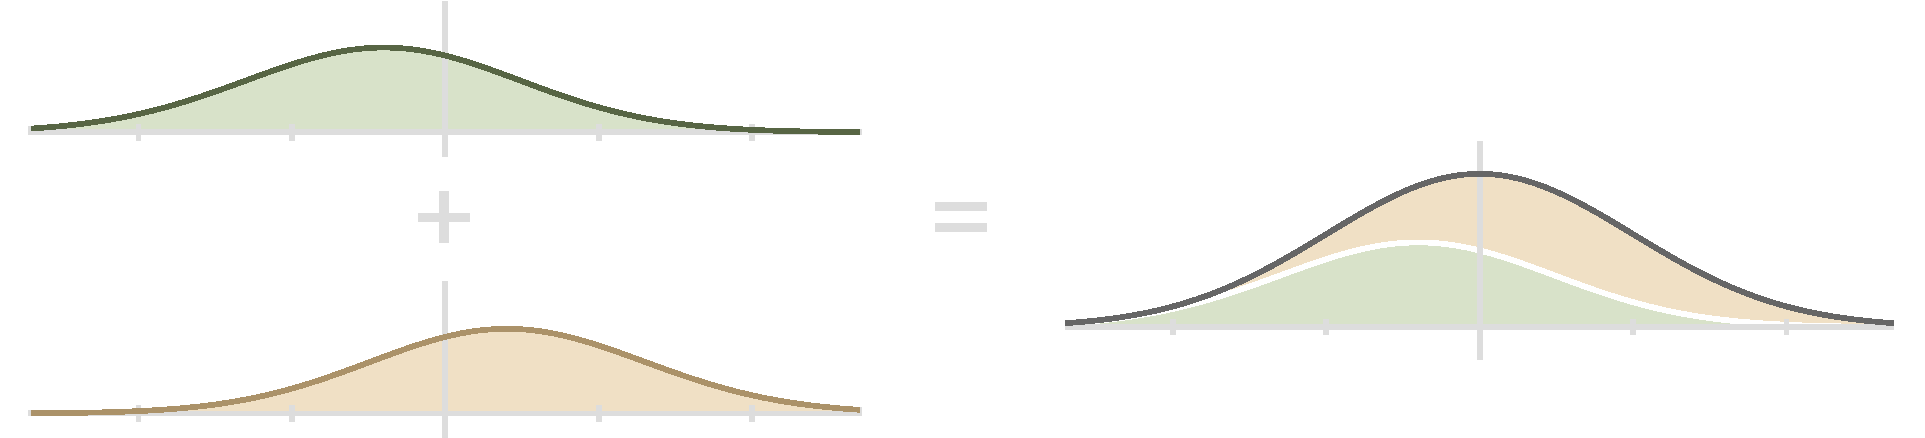
\includegraphics{images/pdfs/added_normals1.pdf}
\caption{The normal curve can be expressed as the sum of two symmetric
normal-like curves.}
\end{figure}

\section{Motivation}\label{motivation}

I became interested in self-replicating functions by working on
algorithms to procedurally generate 3d models of natural-looking trees.
When algorithmically making trees, it makes sense to start from the idea
of an \href{https://en.wikipedia.org/wiki/L-system}{\emph{L-system}},
which can be visualized as a kind of fractal in which a trunk forks into
branches that fork into smaller subranches, this process repeating
infinitely.

I noticed that tree-like \emph{L}-systems can have a large amount of
``branch overlap'' concentrated around a central area of their apparent
surface. For example, consider the two images below. On the left is a
standard \emph{L}-system along with a histogram showing the density of
leaf points along the edge. Intuitively, the leaf points achieve a
reasonable density even toward the extreme angles of the tree's top.
However, the density increases continuously toward the center.

We could think of each leaf point as doing a certain amount of work by
covering some area along the top of the \emph{L}-system. Each subtree is
so oblivious to its other subtrees that they overlap heavily, and the
central leaf points end up being highly redundant. To illustrate this
redundancy, the right-hand figure shows the exact same \emph{L}-system
with essentially half of the tree removed --- yet the shape formed by
the leaf points is only slightly changed.

\begin{figure}[htbp]
\centering
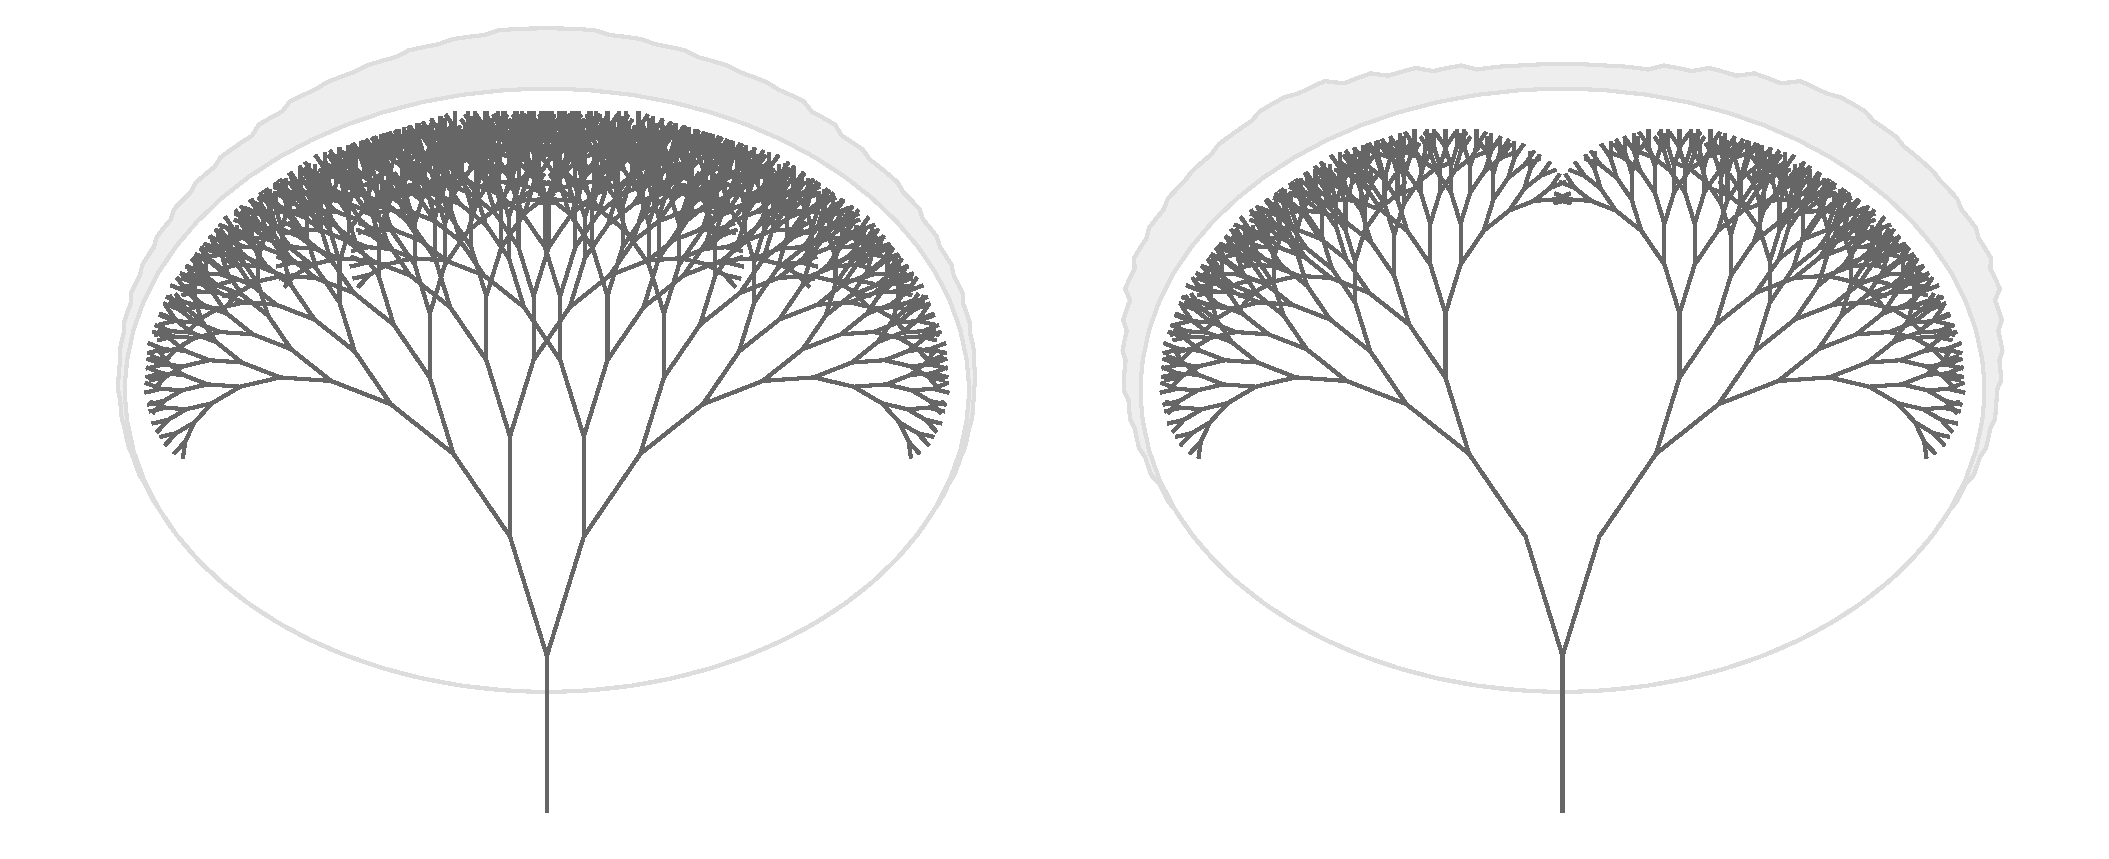
\includegraphics{images/pdfs/ellsystem2.pdf}
\caption{Left: An \emph{L}-system; Right: the same system with two large
subtrees removed. In both cases, a histogram of leaf point density is
provided around an outer ellipse.}
\end{figure}

One approach to smoothing out the distribution of leaf points would be
to compromise the fractal-like nature of the system by choosing each
line direction based on where it is within the fractal, rather than
simply by making each branching point a smaller version of its parent.
The line directions can be chosen so that the set of points at a fixed
distance from the trunk point form a set of equidistant angles from a
central point. The result is an extremely regular edge, as seen below.

\begin{figure}[htbp]
\centering
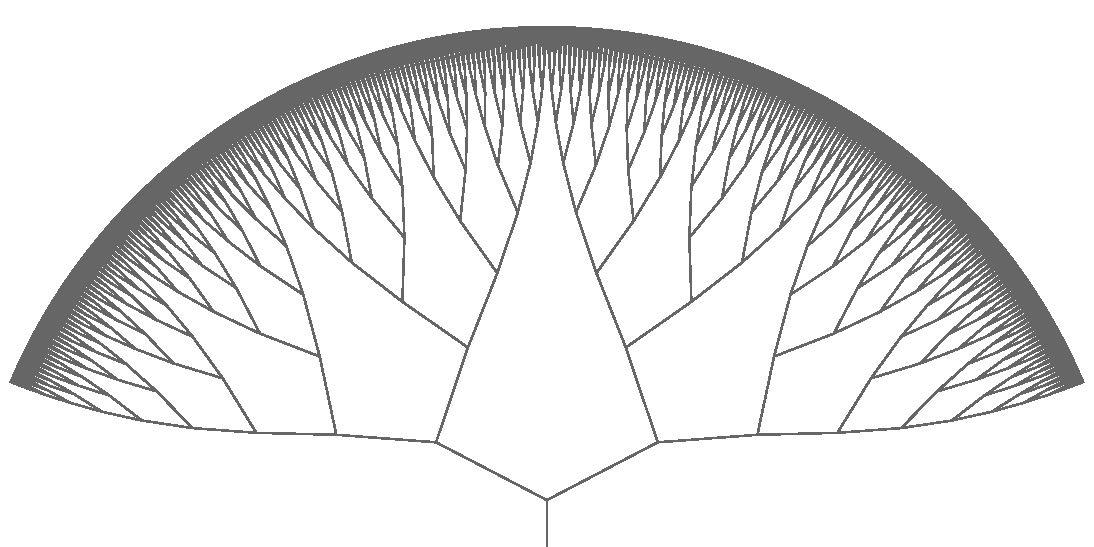
\includegraphics{images/pdfs/well_distributed_ell_like_system.pdf}
\caption{A \emph{L}-like system in which line directions are chosen to
maximize the regularity of leaf point distribution.}
\end{figure}

This is ideally efficient in that each leaf point is equally important
in forming the shape of the system. However, this system is defined in
terms of the path to each point. Is it possible to design a system so
that the overall distribution of leaf points is fairly even, yet each
subtree's shape is independent of its position within the full tree?

If this goal were achieved, we would necessarily have a leaf point
distribution which was the sum of two smaller versions of itself.
Intuitively, the leaf-point distribution of any \emph{L}-system is
already a self-replication function because, if its two main subtrees
have distribution functions \(g_1\) and \(g_2\), then the full tree has
distribution function \(f = g_1 + g_2\). I have to say
\emph{intuitively} here because I haven't formally defined the
leaf-point distribution of an \emph{L}-system.

Thus, \emph{L}-systems naturally coincide with self-replicating
functions. Although there are probably self-replicating functions which
do not correspond with \emph{L}-systems, I nonetheless find it
interesting to independently explore the world of self-replicating
functions.

\section{Simple cases}\label{simple-cases}

Technically, any polynomial can be seen as a kind of self-replicating
function. For example, if \(f(x) = x^2\),

\[\begin{array}{rcl}
  g_1(x) & = & (x + 1)^2 - 1 = x^2 + 2x, \quad \text{and} \\
  g_2(x) & = & (x - 1)^2 - 1 = x^2 - 2x, \\
\end{array}\]

then \(f = g_1 + g_2\), and each \(g_i\) is a shift of the original
function \(f\). In general, if \(f(x) = ax^n + O(x^{n-1})\) then we can
choose \(g_i(x) = a(x\pm 1)^n + O(x^{n-1})\) so that \(f = g_1 + g_2\),
and each \(g_i\) has

\[ \lim_{x\to\pm\infty}\frac{g_i(x)}{f(x)} = 1,\]

which is good enough for me to subjectively say that they strongly
resemble shifts of \(f\).

However, the original motivation for self-replicating functions is based
on distribution functions, so the rest of this note focuses on functions
\(f\) for which \(\lim_{x\to\pm\infty}f(x) = 0\).

Another simple approach would be to set \(g_1 = g_2 = \frac{1}{2}f\) for
any function \(f\). This is not very interesting, and the word
\emph{shift} in the informal definition of a self-replicating function
is intended to defeat this trivial case. That is, each \(g_i\) is
expected to be similar to a translation of \(f\), such as \(f(x-1)\) or
\(f(x+1)\).

The next function I'll describe is simple and meets all of the
requirements so far. An \emph{indicator function} is a function taking
on only the value 0 or 1; it's also sometimes referred to as a
\emph{characteristic function}. If \(f\) is an indicator function, then
you can think of those \(x\) with \(f(x) = 1\) as belonging to the
subset of the domain which is \emph{indicated} by the function. It's
handy to use the following bracket notation of Knuth and others: given
any boolean predicate \(P(x)\), let \([P(x)]\) denote the value 1 when
\(P(x)\) is true, and false otherwise (Knuth 1998).

Given a half-open interval \([a, b)\), define \(I_{[a, b)}\) to be the
function \([x\in[a, b)]\). The following equation shows how such
indicator functions can be considered simple self-replicating functions:
\(I_{[0, 2)} = I_{[0, 1)} + I_{[1, 2)}\).

\begin{figure}[htbp]
\centering
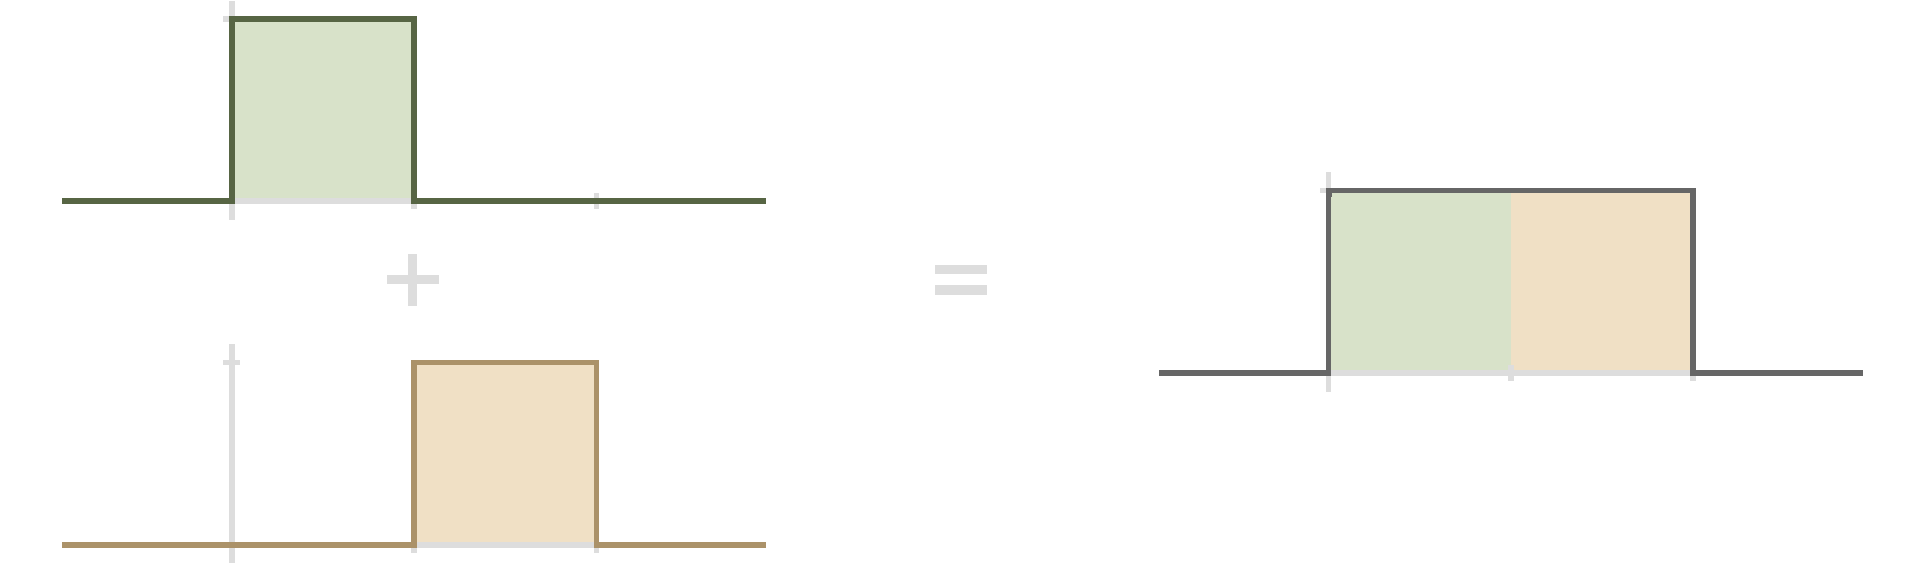
\includegraphics{images/pdfs/added_intervals4.pdf}
\caption{Visual representation of the addition of indicator functions of
intervals.}
\end{figure}

In order to match the equation \(f = g_1 + g_2\), emphasizing the
similarity between the \(g_i\)'s and \(f\), we can set
\(f = I_{[0, 2)}\), \(g_1 = f(2x) = I_{[0, 1)}\), and
\(g_2 = f(2(x - 1)) = I_{[1, 2)}\).

Things get more interesting when \(g_1(x) g_2(x) \ne 0\) for some \(x\).
To this end, define the \emph{ramp function} for values \(a,b,c,d\) with
\(a < b < c < d\) via

\[ J_{a,b,c,d} = \begin{cases}
(x - a) / (b - a) & \text{if } x \in [a, b), \\
1 & \text{if } x \in [b, c), \\
(d - x) / (d - c) & \text{if } x \in [c, d), \text{and} \\
0 & \text{otherwise.} \\
\end{cases}\]

Then \(J_{0,1,4,5} = J_{0,1,2,3} + J_{2,3,4,5}\), as illustrated below.

\begin{figure}[htbp]
\centering
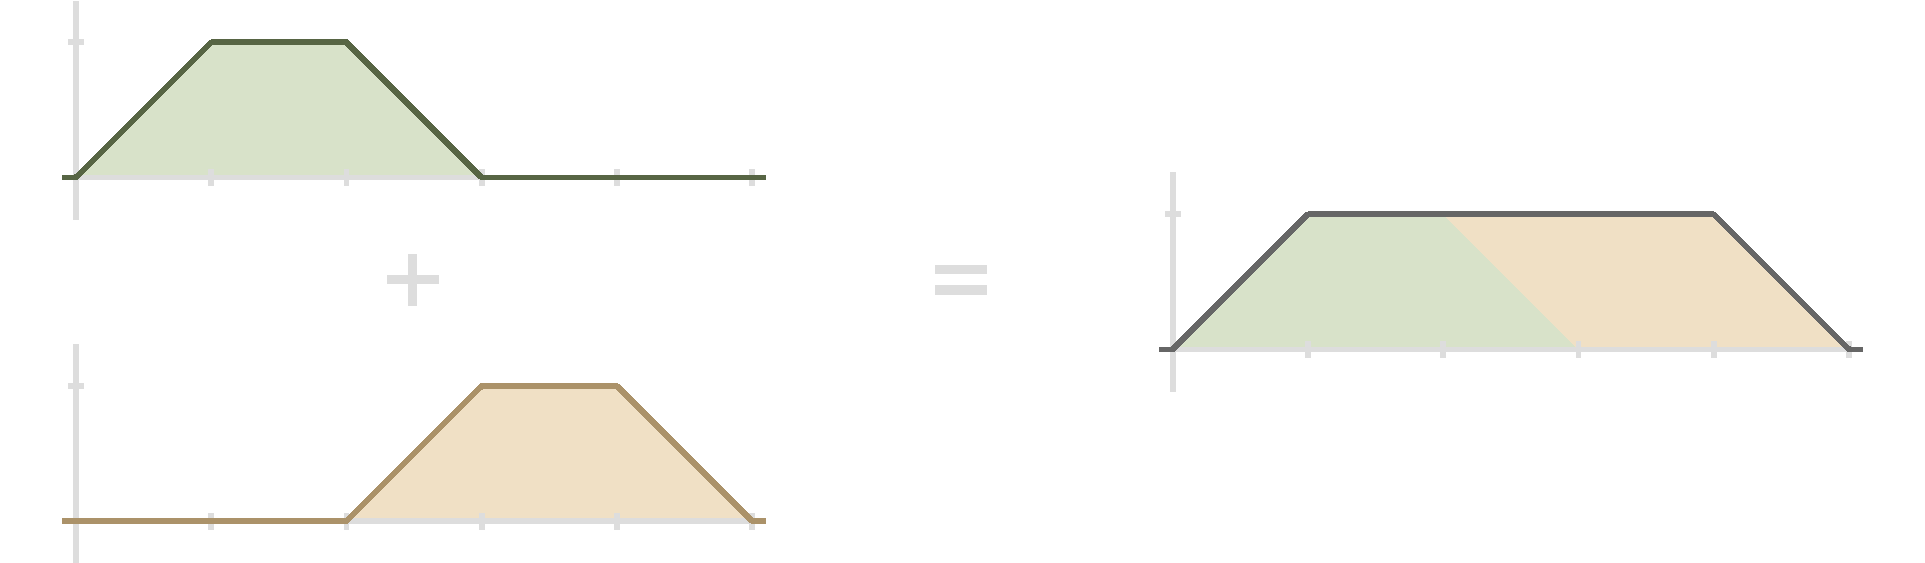
\includegraphics{images/pdfs/ramp_fns.pdf}
\caption{Visual addition of two ramp functions to form another.}
\end{figure}

NEXT up mention that the ramps need not be linear nor symmetric; I'm
interested in exploring fractal-esque, nonflat midsections, even though
this would most likely not be true scales of the sum

\section{The normal curve}\label{the-normal-curve}

The normal curve is described by \(y = e^{-x^2/2}\).

\begin{figure}[htbp]
\centering
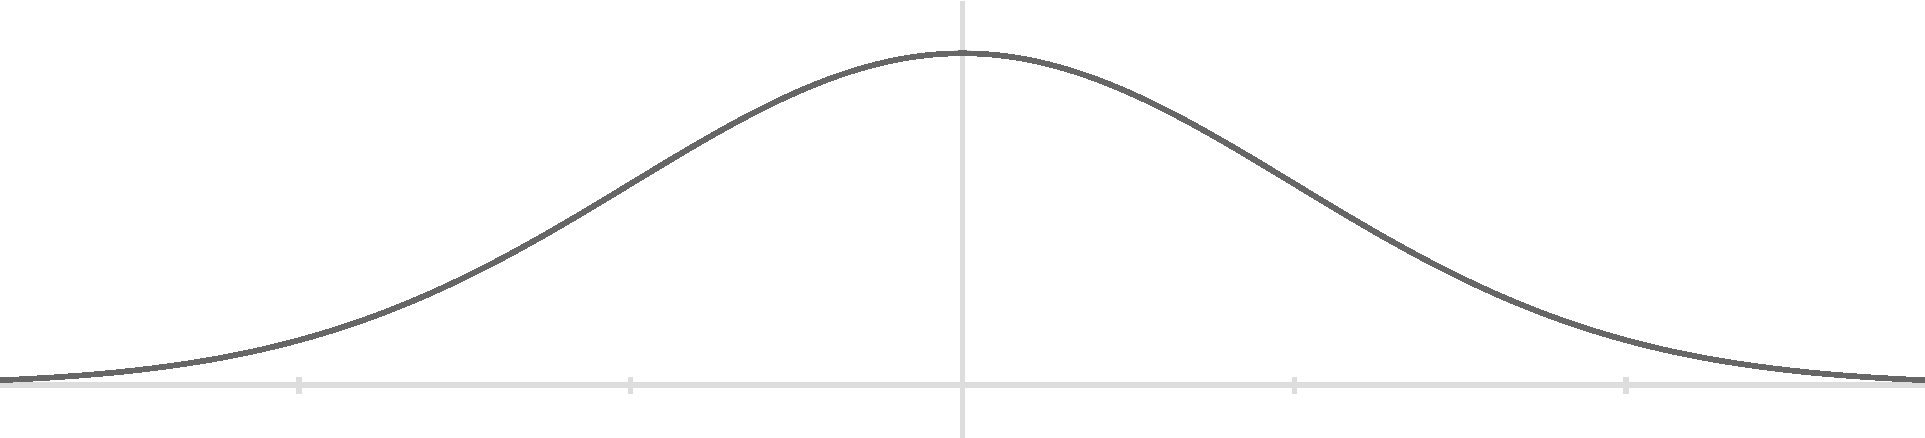
\includegraphics{images/pdfs/normal3.pdf}
\caption{The normal curve: \(y=e^{-x^2/2}\).}
\end{figure}

\section{\texorpdfstring{Leaf-point distributions of
\emph{L}-systems}{Leaf-point distributions of L-systems}}\label{leaf-point-distributions-of-l-systems}

\section{Fractal functions}\label{fractal-functions}

This section is for functions similar to the Cantor diagonal. It may
turn out that I can't find any functions that fit here, or that the
\emph{L}-systems distributions includes this case, or even that I can
prove that no functions could exist here (as far as I know).

\section{Temporary example content}\label{temporary-example-content}

\textbf{Lemma 1}~ \emph{Content of lemma 1, including some \(\pi+3\)
mathy bits.}

\subsection{Subheader}\label{subheader}

Content

See my notes on Raney's lemmas for more examples.

Here is a reference (Knuth, Patashnik, and Graham 1997).

\section{Questions}\label{questions}

\begin{itemize}
\itemsep1pt\parskip0pt\parsep0pt
\item
  The ellipse around my first \emph{L}-system appears to fit
  surprisingly well. Is there a nice way to discover when an ellipse and
  an \emph{L}-system may fit like this? Is there, perhaps, a series of
  shapes which converge on the system or its leaf points, analogous to
  \href{http://mathworld.wolfram.com/MandelbrotSetLemniscate.html}{Mandelbrot
  set lemniscates}?
\item
  The histogram around my first \emph{L}-system appears simple in shape.
  Can its shape be described precisely?
\end{itemize}

\section*{References}\label{references}
\addcontentsline{toc}{section}{References}

Knuth, Donald E. 1998. \emph{Fundamental Algorithms}. Third Ed. Vol. 1.
The Art of Computer Programming. Addison-Wesley.

Knuth, Donald E., Oren Patashnik, and Ronald L. Graham. 1997.
\emph{Concrete Mathematics: A Foundation for Computer Science}.
Addison-Wesley.

\end{document}
